\chapter{位置センサレス位置制御}

\section{センサレスの有効性}上述したように今回のリフトのような位置制御を行う場合,通常,モータの回転角度を検出するロータリーエンコーダを使用して移動量を算出する.しかし,ロータリーエンコーダを使用するにはそれ専用の取付部を新しく設計し取り付けるか,既にロータリーエンコーダと一体化しているモータを購入し使用する必要がある.ロータリーエンコーダを取り付けるにはブラケットや軸継手が必要になり,さらに取付精度も要求される.一体化されたモータなら精度は確保されているが,一般に高価である.
このように,ロータリーエンコーダを後から取り付ける場合は金銭的,時間的にコストがかかる場合が多い.今回提案する位置制御はロボットに取り付ける専用のパーツを使わないため,実現できればそれらのコストを減らすことができる.

\section{センサレス制御の方法}
モータの電流,電圧,回転速度には相関があり,二つの値が定まると残りの一つの値も定まる.電圧の値は操作量なので既知であるため,電流の値が取得できれば,モータの回転速度を求め,それを積分して回転角度を求め,そこから移動量を算出することが出来る.必要なものは電流センサを使った電流計測回路のみなので,ロータリーエンコーダを使うよりも後付けを簡単に行うことができる.

\subsection{制御対象のモデル}
リフトの簡略モデルを図\ref{fig:liftModel}に示す.リフトの運動方程式は式(\ref{eq:lift})のようになる.

\begin{figure}[htbp]
  \begin{center}
    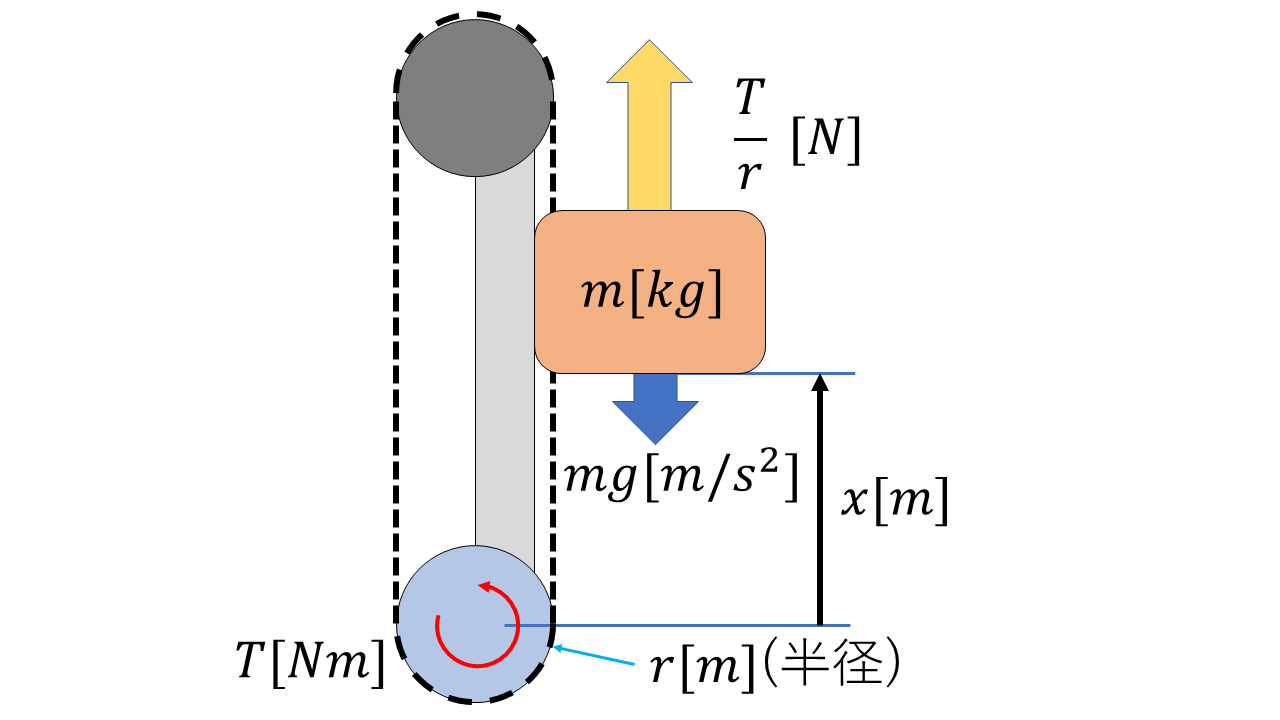
\includegraphics[width=170mm]{img/liftModel.png}
    \end{center}
  \caption{リフトの簡略モデル}
 \label{fig:liftModel}
\end{figure}

\begin{eqnarray}
m\dot{v}=\frac{T}{r}-mg\\
\label{eq:lift}
\end{eqnarray}

式(\ref{eq:lift})をトルクについて変形すると,式(\ref{eq:lift2})のようになる.

\begin{eqnarray}
T=rm(\dot{v}+g)\\
\label{eq:lift2}
\end{eqnarray}

モータ回路の簡略モデルを図\ref{fig:circuitModel}に示す.モータの運動方程式は式(\ref{eq:motor})のようになる.

\begin{figure}[htbp]
  \begin{center}
    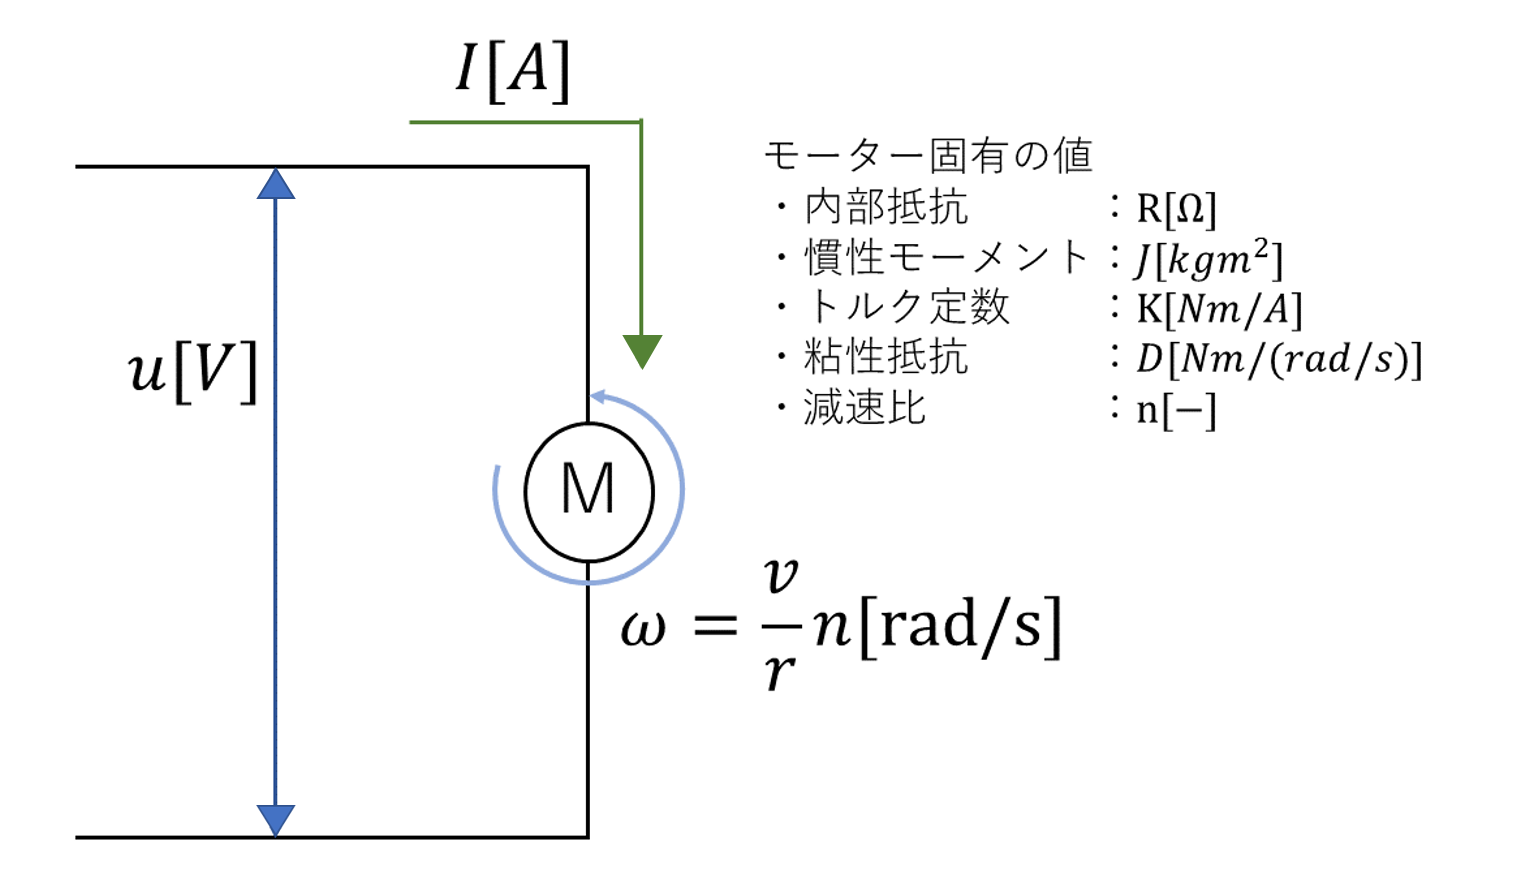
\includegraphics[width=150mm]{img/circuitmodel.png}
    \end{center}
  \caption{モータ回路簡略モデル}
 \label{fig:circuitmodel}
\end{figure}

\begin{eqnarray}
RI+K{\omega}=c\\
J\dot{\omega}+\frac{D}{n}{\omega}-\frac{T}{n}=KI
\label{eq:motor}
\end{eqnarray}

モータの回転数と歯車比,スプロケット半径との関係は式(\ref{eq:rote-v})で表される.

\begin{eqnarray}
{\omega}=\frac{v}{n}r
\label{eq:rote-v}
\end{eqnarray}

リフトの上昇速度を状態量に,電流値を観測方程式とする状態方程式を立てる.式(\ref{eq:lift}),式(\ref{eq:motor})より,リフトの状態方程式は式(\ref{eq:system})のようになる.

\begin{eqnarray}
%\begin{array}{l}
\dot{v}=-\frac{RD+K^2}{RJ+r^{2}m/n^2}v+\frac{KRn}{RJn^{2}+r^{2}m}u-\frac{g}{Jn^{2}/r^{2}m+1}\\
I=-\frac{Kn}{Rr}v+\frac{1}{R}u
%\end{array}
\label{eq:system}
\end{eqnarray}


\subsection{制御系設計}ブロック線図を図\ref{fig:blocksenzu}に示す.

\begin{figure}[htbp]
  \begin{center}
    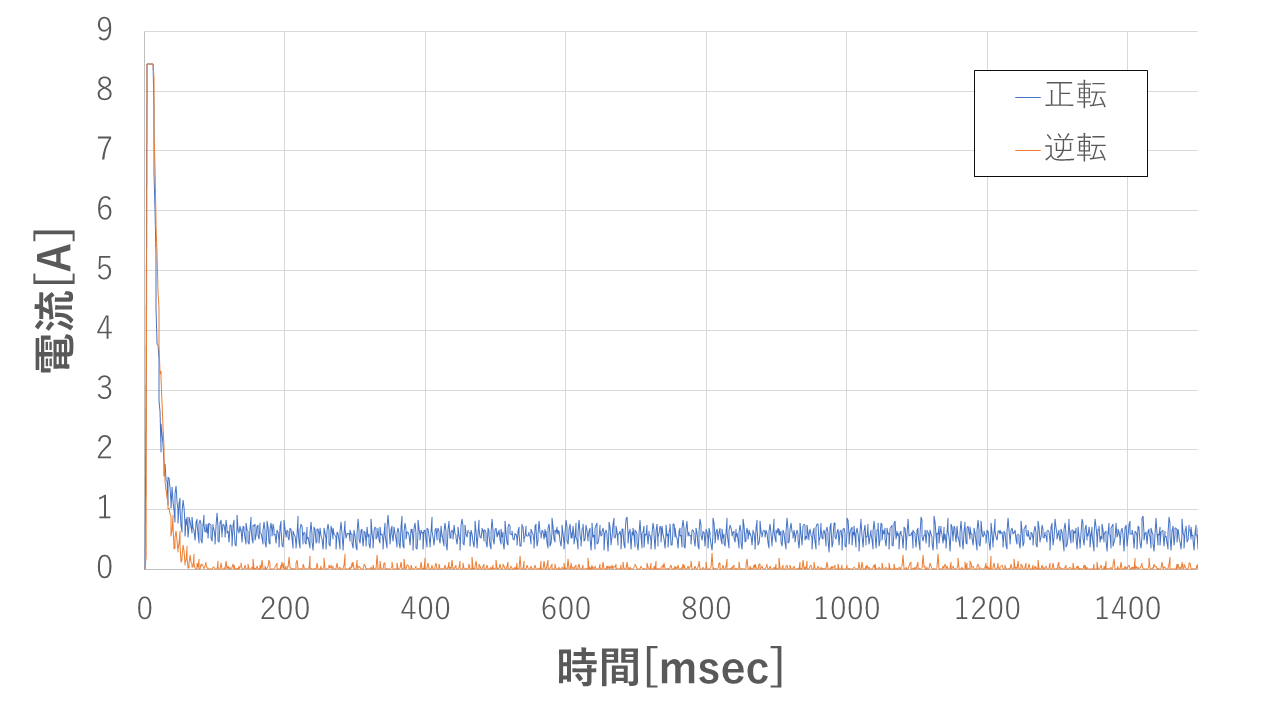
\includegraphics[width=130mm]{img/blocksenzu.png}
    \end{center}
  \caption{ブロック線図}
 \label{fig:blocksenzu}
\end{figure}

リフトには,目標値と現在値の偏差に比例した値を入力する比例制御を行っている.通常の位置制御であればリフトの位置を直接検出してフィードバック制御を行う.しかし今回のセンサレス制御では位置を検出できない.そのため,電流センサから得た電流と入力の電圧から速度測定器でリフトの移動速度を求め,それを積分した値を現在値としてフィードバックする.速度推定器は式(\ref{eq:speed})で表される.

\begin{eqnarray}
v=-\frac{Rr}{Kn}i+\frac{R^2r}{Kn}u
\label{eq:speed}
\end{eqnarray}

速度測定器で算出した移動速度は実際のリフトの移動速度とは異なる可能性がある.
